% Generated by Sphinx.
\documentclass[letterpaper,10pt,english]{manual}
\usepackage[utf8]{inputenc}
\usepackage[T1]{fontenc}
\usepackage{babel}
\usepackage{times}
\usepackage[Bjarne]{fncychap}
\usepackage{longtable}
\usepackage{sphinx}


\title{Cloud Files Introduction Documentation}
\date{August 12, 2009}
\release{1.1.0}
\author{Ranjit Nayak}
\newcommand{\sphinxlogo}{}
\renewcommand{\releasename}{Release}
\makeindex

\newcommand\PYGZat{@}
\newcommand\PYGZlb{[}
\newcommand\PYGZrb{]}
\newcommand\PYGaz[1]{\textcolor[rgb]{0.00,0.63,0.00}{#1}}
\newcommand\PYGax[1]{\textcolor[rgb]{0.84,0.33,0.22}{\textbf{#1}}}
\newcommand\PYGay[1]{\textcolor[rgb]{0.00,0.44,0.13}{\textbf{#1}}}
\newcommand\PYGar[1]{\textcolor[rgb]{0.73,0.38,0.84}{#1}}
\newcommand\PYGas[1]{\textcolor[rgb]{0.25,0.44,0.63}{\textit{#1}}}
\newcommand\PYGap[1]{\textcolor[rgb]{0.78,0.36,0.04}{#1}}
\newcommand\PYGaq[1]{\textcolor[rgb]{0.38,0.68,0.84}{#1}}
\newcommand\PYGav[1]{\textcolor[rgb]{0.00,0.44,0.13}{\textbf{#1}}}
\newcommand\PYGaw[1]{\textcolor[rgb]{0.13,0.50,0.31}{#1}}
\newcommand\PYGat[1]{\textcolor[rgb]{0.32,0.47,0.09}{#1}}
\newcommand\PYGau[1]{\textcolor[rgb]{0.13,0.50,0.31}{#1}}
\newcommand\PYGaj[1]{\textcolor[rgb]{0.00,0.44,0.13}{#1}}
\newcommand\PYGak[1]{\textcolor[rgb]{0.14,0.33,0.53}{#1}}
\newcommand\PYGah[1]{\textcolor[rgb]{0.00,0.13,0.44}{\textbf{#1}}}
\newcommand\PYGai[1]{\textcolor[rgb]{0.73,0.38,0.84}{#1}}
\newcommand\PYGan[1]{\textcolor[rgb]{0.00,0.44,0.13}{\textbf{#1}}}
\newcommand\PYGao[1]{\textcolor[rgb]{0.25,0.44,0.63}{\textbf{#1}}}
\newcommand\PYGal[1]{\colorbox[rgb]{1.00,0.94,0.94}{\textcolor[rgb]{0.25,0.50,0.56}{#1}}}
\newcommand\PYGam[1]{\textbf{#1}}
\newcommand\PYGab[1]{\textit{#1}}
\newcommand\PYGac[1]{\textcolor[rgb]{0.25,0.44,0.63}{#1}}
\newcommand\PYGaa[1]{\textcolor[rgb]{0.19,0.19,0.19}{#1}}
\newcommand\PYGaf[1]{\textcolor[rgb]{0.25,0.50,0.56}{\textit{#1}}}
\newcommand\PYGag[1]{\textcolor[rgb]{0.13,0.50,0.31}{#1}}
\newcommand\PYGad[1]{\textcolor[rgb]{0.25,0.44,0.63}{#1}}
\newcommand\PYGae[1]{\textcolor[rgb]{0.13,0.50,0.31}{#1}}
\newcommand\PYGaZ[1]{\textcolor[rgb]{0.02,0.16,0.45}{\textbf{#1}}}
\newcommand\PYGbf[1]{\textcolor[rgb]{0.40,0.40,0.40}{#1}}
\newcommand\PYGaX[1]{\textcolor[rgb]{0.00,0.44,0.13}{#1}}
\newcommand\PYGaY[1]{\textcolor[rgb]{0.25,0.44,0.63}{#1}}
\newcommand\PYGbc[1]{\textcolor[rgb]{0.00,0.44,0.13}{\textbf{#1}}}
\newcommand\PYGbb[1]{\textcolor[rgb]{0.13,0.50,0.31}{#1}}
\newcommand\PYGba[1]{\textcolor[rgb]{0.00,0.00,0.50}{\textbf{#1}}}
\newcommand\PYGaR[1]{\textcolor[rgb]{0.73,0.38,0.84}{#1}}
\newcommand\PYGaS[1]{\textcolor[rgb]{0.25,0.50,0.56}{\textit{#1}}}
\newcommand\PYGaP[1]{\textcolor[rgb]{0.25,0.44,0.63}{#1}}
\newcommand\PYGaQ[1]{\textcolor[rgb]{0.13,0.50,0.31}{#1}}
\newcommand\PYGaV[1]{\textcolor[rgb]{0.05,0.52,0.71}{\textbf{#1}}}
\newcommand\PYGaW[1]{\textcolor[rgb]{0.25,0.44,0.63}{#1}}
\newcommand\PYGaT[1]{\textcolor[rgb]{0.50,0.00,0.50}{\textbf{#1}}}
\newcommand\PYGaU[1]{\textcolor[rgb]{0.00,0.44,0.13}{#1}}
\newcommand\PYGaJ[1]{\textcolor[rgb]{0.25,0.44,0.63}{#1}}
\newcommand\PYGaK[1]{\textcolor[rgb]{0.02,0.16,0.49}{#1}}
\newcommand\PYGaH[1]{\fcolorbox[rgb]{1.00,0.00,0.00}{1,1,1}{#1}}
\newcommand\PYGaI[1]{\textcolor[rgb]{0.56,0.13,0.00}{#1}}
\newcommand\PYGaN[1]{\textcolor[rgb]{0.05,0.52,0.71}{\textbf{#1}}}
\newcommand\PYGaO[1]{\textcolor[rgb]{0.78,0.36,0.04}{\textbf{#1}}}
\newcommand\PYGaL[1]{\textcolor[rgb]{0.73,0.73,0.73}{#1}}
\newcommand\PYGaM[1]{\textcolor[rgb]{0.00,0.44,0.13}{#1}}
\newcommand\PYGaB[1]{\textcolor[rgb]{0.00,0.25,0.82}{#1}}
\newcommand\PYGaC[1]{\textcolor[rgb]{0.33,0.33,0.33}{\textbf{#1}}}
\newcommand\PYGaA[1]{\textcolor[rgb]{0.00,0.44,0.13}{#1}}
\newcommand\PYGaF[1]{\textcolor[rgb]{1.00,0.00,0.00}{#1}}
\newcommand\PYGaG[1]{\textcolor[rgb]{0.73,0.38,0.84}{#1}}
\newcommand\PYGaD[1]{\textcolor[rgb]{0.25,0.50,0.56}{\textit{#1}}}
\newcommand\PYGaE[1]{\textcolor[rgb]{0.63,0.00,0.00}{#1}}
\newcommand\PYGbg[1]{\textcolor[rgb]{0.44,0.63,0.82}{\textit{#1}}}
\newcommand\PYGbe[1]{\textcolor[rgb]{0.25,0.44,0.63}{#1}}
\newcommand\PYGbd[1]{\textcolor[rgb]{0.00,0.44,0.13}{\textbf{#1}}}
\newcommand\PYGbh[1]{\textcolor[rgb]{0.00,0.44,0.13}{\textbf{#1}}}
\begin{document}

\maketitle
\tableofcontents




\chapter{Introduction}

The Rackspace Cloud Files™ is an affordable, redundant, scalable, and
dynamic storage service offering.  The core storage system is designed
to provide a safe, secure, automatically re-sizing and network accessible
way to store data.  You can store an unlimited quantity of files and each
one can be as large as 5 gigabytes. Users can store as much as they want
and pay only for storage space they actually use.

Additionally, Cloud Files provides a simple yet powerful way to publish
and distribute content behind the industry leading Limelight Networks'
Content Distribution Network. Cloud Files users get access to this network
automatically without having to worry about contracts, additional costs,
or technical hurdles.

Cloud Files allows users to store/retrieve files and CDN-enable content
via a simple Web Service (ReST: Representational State Transfer) interface.
There are also language-specific API’s that utilize the ReST API but make
it much easier for developers to integrate into their applications.

For more details on the Cloud Files service please refer to
\href{http://www.rackspacecloud.com/cloud\_hosting\_products/files}{http://www.rackspacecloud.com/cloud\_hosting\_products/files}


\chapter{Ideal uses of Cloud Files}

There are a number of uses for the Cloud Files service. Cloud Files is an
excellent storage solution for a number of scenarios and is well suited
for a number of applications such as:
\begin{itemize}
\item {} 
Backing up or archiving data

\item {} 
Serving images/videos (streaming data to the user's browser)

\item {} 
Serving content with a world-class CDN (Limelight Networks)

\item {} 
Storing secondary/tertiary, static web-accessible data

\item {} 
Developing new applications with data storage integration

\item {} 
Storing data when predicting storage capacity is difficult

\item {} 
Storing data for applications affordably

\end{itemize}


\chapter{Why use Cloud Files}

There are a number of reasons to choose the Cloud Files service over
similar services available in the market.
\begin{itemize}
\item {} 
Simplicity of security mechanisms and CDN functionality

\item {} 
Affordability of the service with a price of just 15cents / gigabyte of storage

\item {} 
Flexibility in terms paying as you go

\item {} 
Several developer programming interfaces

\item {} 
Great performance

\item {} 
World class support

\end{itemize}


\chapter{Cloud Files Features}


\section{Simplicity}

Cloud Files is simple to use for developers and non-developers alike.
Users can get started in as little as five minutes. Users do not have
to know how to code to use Cloud Files and CDN.  Users can, within
minutes, sign up for Cloud Files, create a Container, upload a file and
publish that Container’s content through the CDN (Refer to “Cloud Files
with CDN QuickStart guide”. The Cloud Files GUI is easy to navigate and
use. Rackspace browser based control panel let users easily upload files
and distribute on a CDN without writing any code.

All the content can be backed by a CDN without complex negotiations and
details of updating content for optimizing delivery.  Given the complexity
of the CDN, users may have to make a series of choices such as number of
servers to use etc. before obtaining the service.  After making the choices
users must ensure the usage bills are accurate.  All these issues are
handled by Cloud Files. CDNs have, in the past, been the prerogative of
companies with more money but Cloud Files has changed that.

Cloud Files is a user and developer friendly service. Security mechanisms
described in more detail in the Security section are simple to use. Third
party tools which further simplify use of the storage service are available.
Developers can use a language specific application programming interfaces
to develop utilities or applications.  The API’s are easy to use and are
documented with examples to get started quickly.


\section{Affordability}

Pricing for Cloud Files with CDN starts at 15 cents per gigabyte of storage
and 8 cents per gigabyte inbound and 22 cents per gigabyte of bandwidth
outbound to any edge location around the globe. There are no per requests
fees for CDN. For the latest pricing information please refer to the Cloud
Files web site.


\section{Flexibility}

Cloud Files is a dynamically expanding storage system very flexible and is
built on the pay for use principle. Customers can use as much or little
storage as necessary, while paying only for storage space used. There is
no limit on total space use and individual files can be as large as 5GB.
The GUI control panel allows users to check storage space used and
bandwidth utilized. There are no upfront fees or contracts and end users
pay only for storage space used and outgoing bandwidth that they use.

System administrators can use this for simple manual updates as well.
Users do not have to know how to code to use Cloud Files and CDN.  No API
is required to share files.  Non-developers have a simple web-interface,
that can be used to quickly and easily upload data and enable CDN access.
There are multiple third party tools (refer to Tools and Applications
section) which make it even more flexible for users of specific
environments such as the Mac OS.

Developers can use the ReST web service and language-speicifc API’s in
PHP, Python, Java, Ruby, and C\#/.NET.  The API's provide full support for
managing content in Cloud Files and publishing content over the CDN. The
API allow developers to work in the language they feel most comfortable


\section{Superior performance}

Rackspace has built networks with superior performance for years. The
Limelight Networks CDN capability improves the performance further for
distribution of digital content. Limelight’s scale has no individual
limits.  Maximum transfer speed and requests per second are only limited
by the overall, aggregate egress capacity of Limelight’s network which,
at this time is 2.2Tbps. In short, Limelight can bring data closer to
end users and serve popular content faster. To test the performance,
8KB files were placed in Cloud Files.  Then Gomez was used to measure
end to end response times (including DNS resolution, etc.) to the content
via the CDN URLs, every five minutes, over the course of one week, from
various nodes throughout the world.  The average response time in the US
was 57ms for Cloud Files.  The average response time from global locations
was 107ms for Cloud Files. For more details and comparisons with similar
services please refer to blog entries on the Rackspace Cloud blog. For more
information on why CDNs improve performance please refer to the document
titled “Content Delivery Networks with Cloud Files”.


\section{World Class support}

With Cloud Files world-class free technical support is only a click away.
Live support, with real people is available 24/7.  Fanatical Support is
built into the price. Users can get peace of mind knowing that technical
support is just a phone call or online chat away – at any time of the day.


\section{Data Redundancy}

The Cloud Files storage system is designed to be highly available and
fault tolerant.  Cloud Files achieves client data redundancy by
replicating three full copies on different storage nodes.  Storage nodes
are grouped in logical Zones within Rackspace datacenters.  Zones are
connected to redundant Internet backbone providers and reside on redundant
power supplies and generators.  The system has been engineered in such
a way as to continue to by fully functional even in the event of a major
service disruption within a Datacenter. Content on the CDN provides an
additional layer of data redundancy.


\section{Security}

Cloud Files uses a number of different measures to ensure that your data
is kept safe. First and foremost, all traffic between clients and the
Cloud Files system uses SSL to establish a secure, encrypted communication
channel. This ensures that any data (usernames, passwords, and content)
cannot be intercepted and read by a third-party.  Users authenticate with
a valid username and API Access Key and are granted a session authentication
token. These authentication tokens are used to validate all operations
against Cloud Files. There is no way to terminate a valid session by the
user, but the session tokens will automatically expire after 24 hours,
forcing clients to resend their credentials.

The API Access Key is only available from within the Rackspace Cloud’s web
control panel at \href{http://www.rackspacecloud.com}{http://www.rackspacecloud.com}.  Users must enter their valid
username and password to gain access to view the API Access Key or to
generate a new key.

It is important to note that Cloud Files does not apply any transformations
to data before storing it. This means that Cloud Files \emph{will not} store data
in encrypted form unless the client encrypts it prior to transmission. This
allows users to select the type and level of encryption best suited for
their application.

When deleting storage Objects from the Cloud Files system, all copies of
data are permanently removed within a matter of minutes.  Furthermore,
the physical blocks making up the customer’s data is zeroed over before
that space is re-used for other customer data. In other words, after a
delete request, the data will be unrecoverable.


\chapter{Tools and Applications for Cloud Files}

In addition to the ReST and language API's, there are several other ways
for users to interact with Cloud Files.


\section{Control Panel}

The control panel on The Rackspace Cloud’s site is one way to access Cloud
Files. Files can be uploaded and downloaded through the control panel.
This is a tool to understand at a high level how Cloud Files works.  It
gives system administrators a view of the various containers and objects
stored on Cloud Files. It is great GUI tool to update individual files and
metadata on the files.

{\hfill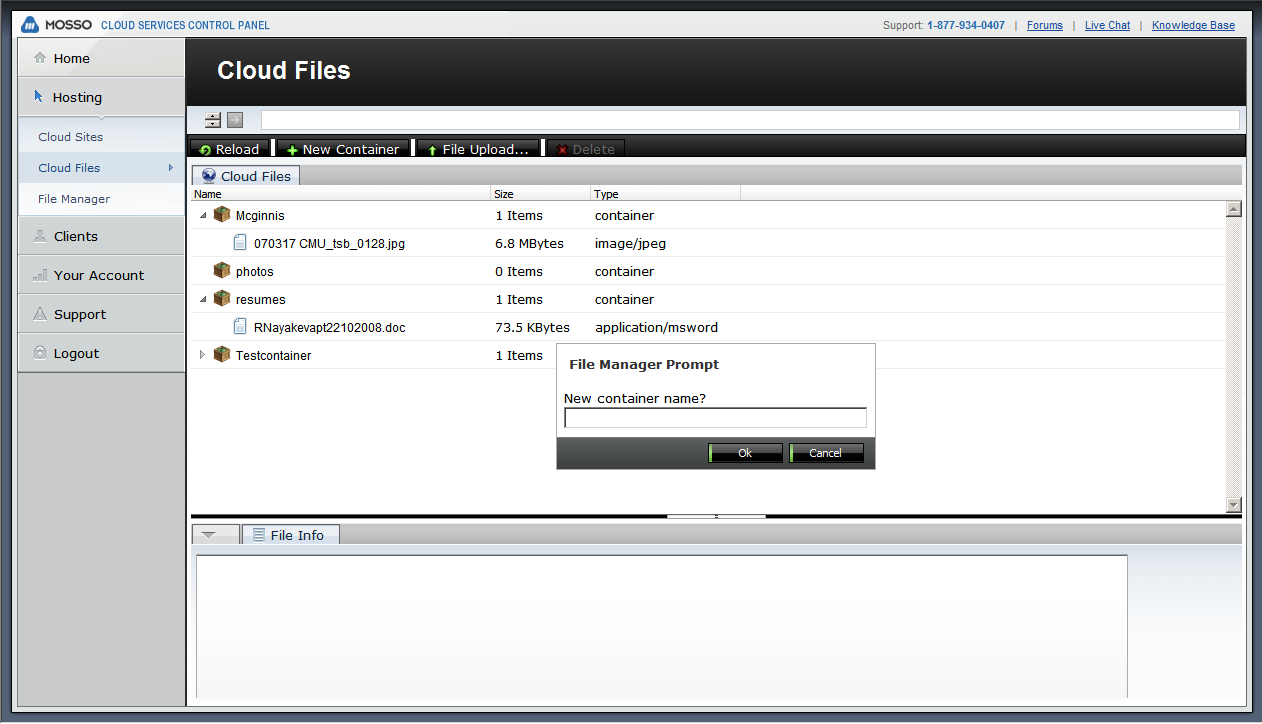
\includegraphics{cp.png}\hfill}


\section{FireUploader}

FireUploader is a tool from Suchi Software and it provides an intuitive
interface to move to and manage files in Cloud Files. It works as a plug-in
to the Mozilla Firefox browser and provides a GUI to manage the movement as
well as meta data in Cloud Files as shown in Figure 2.  While setting up
the tool you must supply your Rackspace Cloud username and when prompted for
a “password’, enter your API Access Key. This tool provides creative way of
working with available Cloud Files features to allow users to simulate a
hierarchical file system structure.  For more information, please see the
\href{http://www.fireuploader.com}{Fireuploader} web site.

{\hfill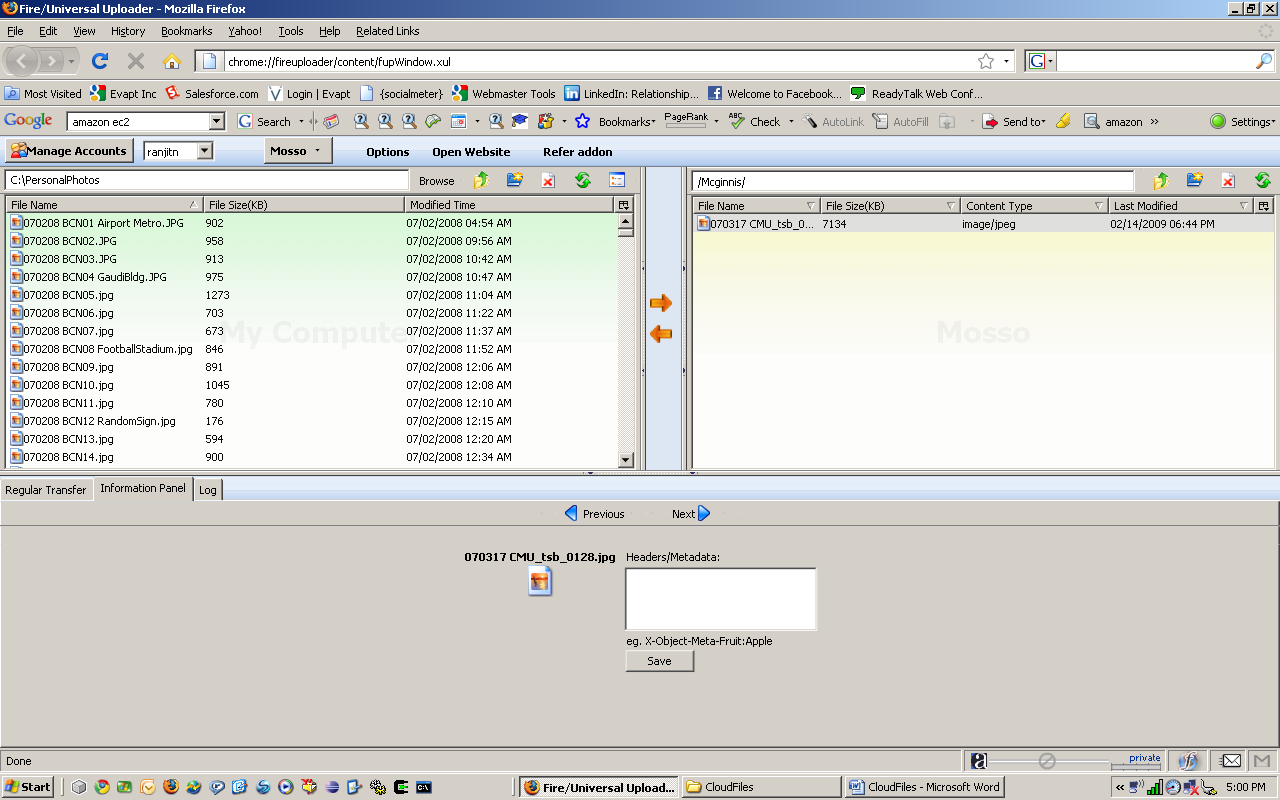
\includegraphics{fireuploader.png}\hfill}


\section{Cyberduck}

Cyberduck is an open source Cloud Files browser licensed under the GPL that
runs on Macs. It features an easy to use interface with easily accessible
bookmarks. The browser outline view allows users to browse large folder
structures efficiently and preview files with Quick Look.  Cyberduck also
provides a seamless integration with many external editors making it easy
to change content quickly.  It provides a way to upload and configure Cloud
Files to distribute content over the CDN.  Cyberduck also supports many OS
X core system technologies such as Spotlight, Bonjour, Keychain and a large
number of language translations. Cyberduck 3.x requires Mac OS X 10.4 or
later.  For more information, please see the \href{http://www.cyberduck.ch}{Cyberduck} web site.

{\hfill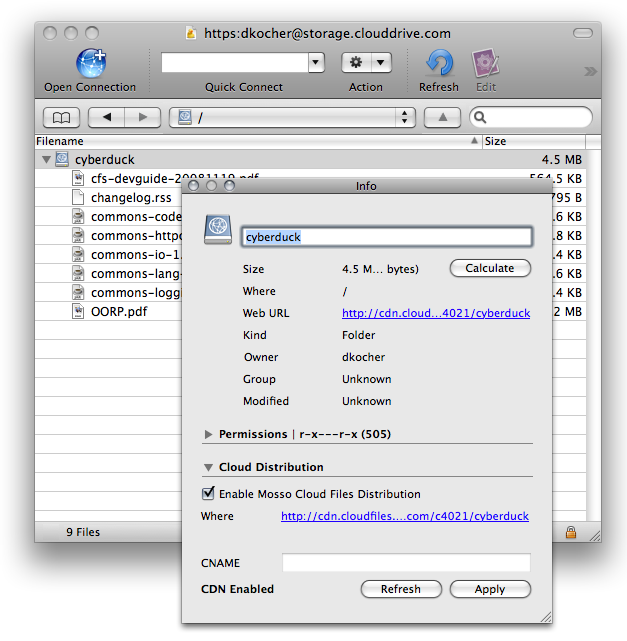
\includegraphics{cyberduck.png}\hfill}


\chapter{Developing applications for Cloud Files}

There are several programming interfaces for using Cloud Files that will
allow developers to integrate the storage solution into new applications,
or provide automated ways of accessing the system. The best way to get
started is to follow the steps enumerated in the QuickStart guide. For
more details on developing applications please refer to “Cloud Files
Developer Guide”.


\section{ReST API}

Cloud Files allows users to store/retrieve files via a simple Web Service
(ReST: Representational State Transfer) interface. New Cloud Files storage
applications such as the tools described in the previous sections can be
designed and developed by using the ReST application programming
interface. The complete API documentation can be found on the Rackspace
Rackspace Cloud web site.


\section{Language specific API}

In addition to the ReST API, there are language specific API documents and
assets for C\#/.NET, Python, PHP, Java and Ruby. For more information please
refer to Developer resources on the Cloud Files web site.


\section{Caveats}

There are many great use-cases and advantages to a storage system like
Cloud Files.  However, there are limitations depending on your needs and
some use-cases where Cloud Files is not an ideal storage solution.  Keep
the following points in mind as you further explore Cloud Files:
\begin{itemize}
\item {} 
Native support within your Operating System. It is not possible to
``mount'' or ``map'' the Cloud Files storage system as a virtual hard-disk
on your computer or server.

\item {} 
Disk mirroring or backup solutions that require byte/block level
differences. There are no concepts of ``appending data'' or ``file locking''
operations within Cloud Files.

\item {} 
Data can be organized into storage compartments called ``Containers'',
but Containers cannot be nested. Since there is only one top-level of
organization, you will not be able to upload a nested directory/folder
structures into Cloud Files unless a transformation is performed to
flatten the structure.

\item {} 
There is no built-in concept of permissions or access controls the Cloud
Files system that you are probably used to in a traditional file system.

\item {} 
There are no transcoding capabilities to read a file in one format and
upload the same into one or more formats into Cloud Files.

\end{itemize}


\chapter{Additional Resources}

The official support channels (phone, chat, email, forums, and knowledge
base articles) for Cloud Files are available at the Rackspace Cloud’s web
site: \href{http://www.rackspacecloud.com}{http://www.rackspacecloud.com}.

There is a temporary system status page available at
\href{http://status.cloudfiles.rackspacecloud.com}{http://status.cloudfiles.rackspacecloud.com} that can be reviewed if you
believe the system is not functioning to your expectations. This page
is updated to reflect up-to-date information about the system's current
health and status.  Over time, Cloud Files users will be directed to a
more comprehensive status page that reflects the system health of all
major cloud products.

Interested users can also follow updates/announcements via twitter at
\href{http://www.twitter.com/cloudfiles}{http://www.twitter.com/cloudfiles}.

IRC savvy developers are also encouraged to join some of the members of
the Cloud Files team at irc.freenode.net on the \#cloudfiles channel.
This is not an official Cloud Files support channel but should rather be
viewed as a community meeting place to share/discuss Cloud Files.


\chapter{Trademarks}

The following terms are trademarks of Rackspace Hosting Inc in the
United States:
\begin{itemize}
\item {} 
Cloud Files

\item {} 
Cloud Servers

\item {} 
Cloud Sites

\end{itemize}

Java™ and all Java-based trademarks are trademarks of Sun Microsystems,
Inc. in the United States, other countries, or both.

Linux® is a registered trademark of Linus Torvalds in the United States,
other countries, or both.

UNIX® is a registered trademark of The Open Group in the United States
and other countries.

Other company, product, and service names may be trademarks or service marks of others.


\renewcommand{\indexname}{Module Index}

\renewcommand{\indexname}{Index}
\printindex
\end{document}
